
\documentclass[english]{article}
\usepackage{graphicx}
\usepackage{amsmath}
\usepackage{hyperref}
\usepackage{setspace}
\usepackage{apacite}
\usepackage{hyperref}
\usepackage{natbib}
\usepackage{pxfonts}
\usepackage[utf8]{inputenc}
\usepackage[left=1in,right=1in,top=1in,bottom=1in]{geometry}
\usepackage[left]{lineno}
\usepackage{soul}
\usepackage{setspace,caption}
\doublespacing
\captionsetup[figure]{labelsep=period,labelfont=it,justification=justified,
 singlelinecheck=false,font=doublespacing}
\usepackage[left=1in,right=1in,top=1in,bottom=1in]{geometry}
\linenumbers

\newcommand{\gazeLocations}{S1}
\newcommand{\excludedTrials}{S2}
\newcommand{\ratingsByCategory}{S3}

\begin{document}


\title{Category-based and location-based volitional covert attention affect
memory at different timescales}

\author{Kirsten Ziman$^1, 2$,
Madeline R. Lee$^1$,
Alejandro R. Martinez$^1$,\\
Ethan D. Adner$^1$,
and
Jeremy R. Manning\textsuperscript{$1, \dagger$}\\[0.1in]$^1$Dartmouth College\\
$^2$Princeton University\\
\textsuperscript{$\dagger$}Address correspondence to jeremy.r.manning@dartmouth.edu}

\maketitle

\begin{abstract} 
  
Our ongoing subjective experiences, and our memories of those experiences, are
shaped by our prior experiences, goals, and situational understanding. These
factors shape how we allocate our attentional resources over different aspects
of our ongoing experiences. These attentional shifts may happen overtly (e.g.,
when we change where we are looking) or covertly (e.g., without any explicit
physical manifestation). Additionally, we may attend to what is happening at a
specific spatial location (e.g., because we think something important is
happening there) or we may attend to particular features irrespective of their
locations (e.g., when we search for a friend's face in a crowd versus a
location on a map). We ran a covert attention experiment with two conditions
that differed in how long they asked participants to maintain the focus of the
categories and locations they were attending. Later, the participants performed
a recognition memory task for attended, unattended, and novel stimuli.
Participants were able to shift the location of their covert attentional focus
more rapidly than they were able to shift their focus of covert attention to
stimulus categories, and the effects of location-based attention on memory were
longer-lasting than the effects of category-based attention.

\noindent\textbf{Keywords: covert attention, spatial attention, category-based
attention, recognition memory, perception}

\end{abstract}


\section*{Introduction} 

Our brains' cognitive systems detect and exploit patterns in our prior and
ongoing experiences, enabling us to function and adapt in an ever-changing
world. However we do not attend to or treat all types of remembered or incoming
information equally, and our ability to flexibly adapt our thinking and
behaviors can vary markedly with the specific set of concepts or tasks relevant
to a given setting or situation~\citep{ChunTurk07, AlyTurk17, HardNade09,
RangRitc12}. There is also substantial variability across people with respect
to which aspects of experience (sensory, social, emotional, etc.) are noticed,
discriminated between, and acted upon~\citep{HuntEtal89}. This implies that the
same physical (objective) experience may give rise to very different perceived
(subjective) experiences across people~\citep{FreeSimo11, ChanEtal18}.

The aspects of our experience we attend may be under our volitional control or
may be unconscious or automatic~\citep{JacoEtal92}. Both volitional and
unconscious attention may be expressed overtly, for example through intentional
eye movements~\citep{HoffSubr95} or covertly, without any volitional physical
change~\citep{EngbKlie03}. Prior work has explored the similarities and
differences in the neural basis of overt versus covert
attention~\citep{PosnEtal87, HuntKing03} as well as the behavioral and neural
underpinnings of volitional versus unconscious attention~\citep{DijkAart10} and
their differential effects on memory. There is a general consensus that
sustained volitional attention enhances memory relative to unconscious
attentional processes~\citep{UncaEtal11, GoloEtal13}. However, volitional
attention takes many forms, such as attention to particular spatial locations
or attention to particular visual features or other stimulus properties. How
different \textit{types} of volitional attention combine (or compete) to
enhance memory remains an open question. Volitional covert attention is of
particular interest in that it allows us to dynamically and intentionally
manipulate our experience, even when our sensory input remains largely
static~\citep[i.e., constant physical stimuli, retinal image, etc.][]{YiEtal06,
OcraEtal99}.

Here we examine the ways different types of volitional covert attention
interact to affect memory. We designed an experimental
paradigm~\citep[following][]{Posn80} that asked participants to attend to a
series of presented composite image pairs while keeping their gaze fixed on a
central point. The image pairs comprised a left and right image, each
constructed by blending an image of a face and place. The stimuli and
presentation durations were constant across the two experiments, but the
experiments differed in how often we asked participants to change the focus of
their attention with respect to image category (face versus place) and image
location (left versus right). After the participants attended to a series of
images, we used a recognition memory test to assess which aspects of the
presented images had been encoded into memory. In both experiments we found
that the images participants covertly attended to were better recognized than
other images, supporting the notion that attention enhances memory
encoding~\citep[i.e., they rated attended images as more familiar than
unattended images][]{Yone02}. After maintaining the focus of attention to a
single image category and location (Sustained Attention Experiment),
participants also recognized the attended-category image at the unattended
location, and (to a lesser extent) the unattended-category image at the
attended location. After more rapidly varying their focus of attention
(Variable Attention Experiment), participants showed a similar boost in
recognition for the unattended-category image at the attended location, but
they did not recognize images at the unattended location. This suggests that
participants were able to shift the location of their covert attentional focus
more rapidly than they were able to shift their focus of covert attention to
stimulus features. We also found differences in the timecourses of these memory
effects, suggesting that the impact of location-based attention on memory
persists on the order of several seconds longer than the impact of
feature-based attention.

\section*{Materials and methods}

We ran a total of 53 participants in across two experimental conditions
(Fig.~\ref{fig:paradigm}). The two conditions differed in how often we
cued participants to change the focus of their attention. All code and
documentation pertaining to our experiments and analyses, along with the
experimental stimuli and data, may be downloaded from
\url{http://www.github.com/ContextLab/attention-memory-task}.

\begin{figure*}[tp]
  \centering
  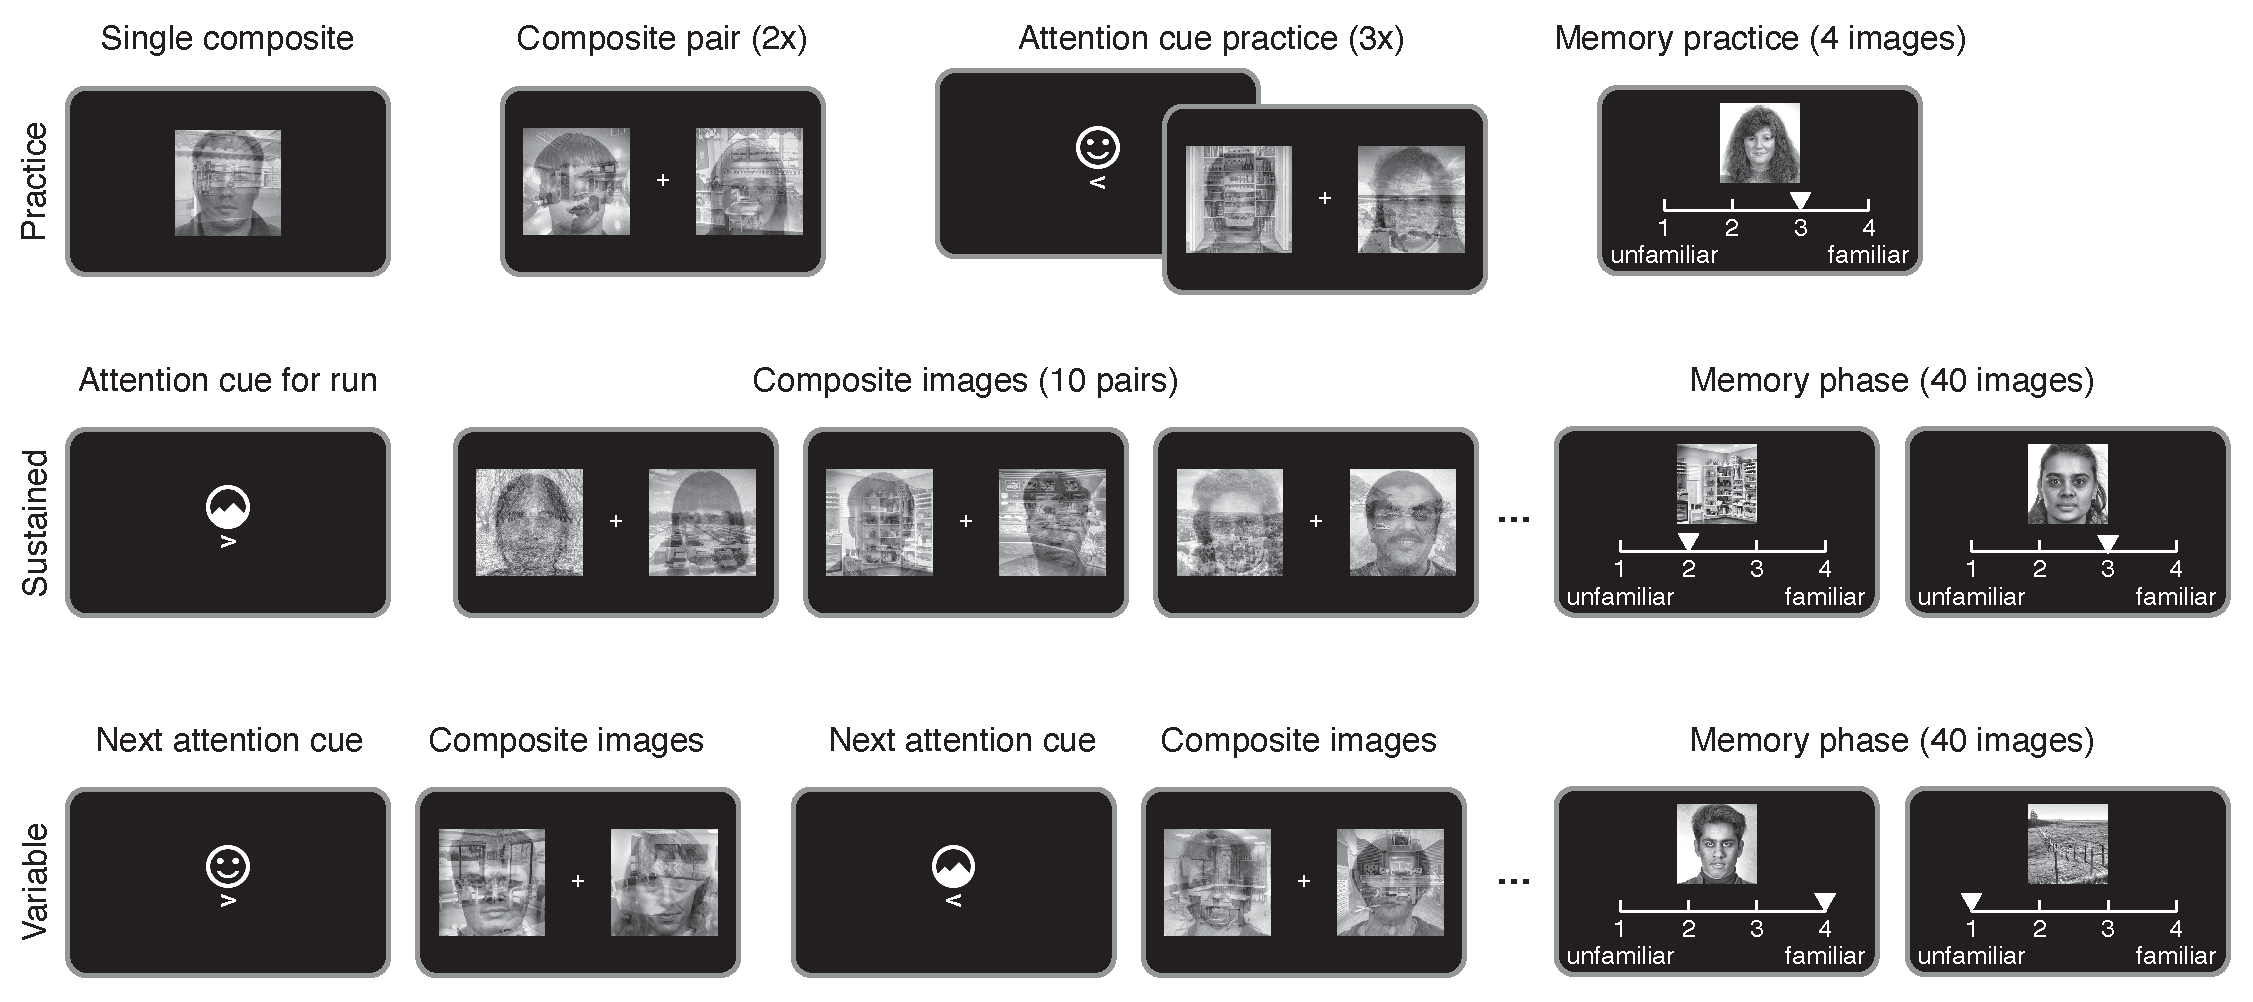
\includegraphics[width=1\textwidth]{figs/paradigm}

  \caption{\textbf{Experimental paradigm.} \textbf{A.--D. Practice phase.}
  \textbf{A.} Composite face/place image. \textbf{B.} A single pair of
  composite images and a central fixation cross. \textbf{C.} One attention cue
  practice trial. \textbf{D.} Familiarity judgement practice trial. \textbf{E.
  Sustained attention condition.} Participants receive an attention cue,
  followed by a sequence of 10 composite image pairs (Panel E), and then they
  make of familiarity judgements on each of 40 face and place images, presented
  in sequence (Panel F).  \textbf{G.  Variable attention condition.}  Participants
  study a succession of 10 composite image pairs, each preceded by an attention cue.
  After studying the images, they make a series of 40 familiarity judgements about
  face and place images, as in the sustained attention condition (Panel F).}

\label{fig:paradigm}
\end{figure*}

\subsection*{Participants} 

A total of 53 Dartmouth College undergraduate students enrolled in our study
(30 in the sustained attention condition and 23 in the variable attention
condition). Following a pilot study using a similar experimental design, we
aimed to enroll 30 participants in each condition. However, we fell short of
our enrollment target in the variable attention condition when in-person
testing was discontinued at our institution due to the COVID-19 pandemic. All
participants had self-reported normal or corrected-to-normal vision, memory,
and attention. Participants gave written consent to enroll in the study under a
protocol approved by the Committee for the Protection of Human Subjects at
Dartmouth College.

We used a voluntary pre-experimental survey to collect self-reported
demographic information about each partipant. All 53 participants elected to
fill out the survey. Participants ranged in age from 18--21 years old (mean:
18.7 years; standard deviation: 0.8 years). Participants reported their genders
as female (34 particiapnts), male (18 participants), and gender non-binary (1
participant). Participants reported their ethnicities as Not Hispanic or Latino
(44 particiapnts), Hispanic or Latino (7 participants), or declined to respond
(2 participant). Participants reported their race as White (37 participants),
Asian (13 participants), American Indian or Alaska Native (4 participants),
Black or African American (2 participants), and Other (1 participant). Note
that each participant could report one or more racial categories, as they
deemed appropriate.

Fourty-nine participants reported having no reading impairments, and 4
participants reported having reading impairments such as dyslexia. Fifty
participants reported having normal color vision and 3 reported having abnormal
color vision such as colorblindness. Fifty participants reported taking no
medications and having no recent injuries. One participant reported that they
had recently ``hit [their] head very hard.'' Another reported having taken
concerta in the past, but mentioned they had not taken it recently. One
participant reported using amphetamines regularly, but also clarified that they
were not currently on amphetamines at the time of testing.

We also asked participants to self-report on their sleep, alertness, and coffee
consumption. Participants reported having gotten between 4 and 9 hours of sleep
on the night prior to testing (mean: 6.9 hours; standard deviation: 1.3 hours).
Participants reported their alertness at the time of testing, and we converted
their responses to point values as follows: ``Very alert'' (5 points), ``A
little alert'' (4 points), ``Neutral'' (3 points), ``A little sluggish'' (2
points), and ``Very sluggish'' (1 point). Across all participants, the full
range of alertness values were used (maximum: 5; minimum: 1; mean: 3.44;
standard deviation: 1.0). Participants reported having consumed between 0 and 2
cups of coffee so far on their testing day (mean: 0.3 cups; standard deviation:
0.5 cups).

\subsection*{Stimulus selection and presentation} 

Participants viewed photographs of faces, places, and composite images each
comprising an equal blend of one face image and one place image. The pool of
360 face images included photographs of adult human male and female faces
selected from the FERET database~\citep{PhilEtal98}. The pool of 360 place
images included photographs of indoor and outdoor places selected from the SUN
database~\citep{XiaoEtal10}. The images we used from both databases came from a
stimulus subset that was manually curated by Megan deBettencourt (personal
communication). All images were resized to $256 \times 256$ pixels, converted
to greyscale, and processed so that every image was matched for mean contrast
and intensity. We selected 20 face images and 20 place images from the stimulus
pool to use in the instructional and practice phases of the experiments
(Fig.~\ref{fig:paradigm}A--D).

In addition to the face and place images, we presented (in white) attention
cues to direct the participant's focus of attention. The attention cues
comprised a stylized icon of a face or mountain peaks, directing attention to
the face or place component of the images, respectively; and a left- or
right-facing angled bracket, directing attention to the left or right image,
respectively (e.g., Figs.~\ref{fig:paradigm}C, E, and G).

 Our experiment was conducted in a sound- and light-attenuated testing room
 containing a chair, desk, and 27-inch iMac desktop computer (display
 resolution: $2048 \times 1152$). The participant sat in the chair and rested
 their chin on a chin rest located 60~cm from the display. The active portion
 of the display screen occupied 52.96$^\circ$ (width) and 31.28$^\circ$
 (height) of the participant's field of view from the chin rest. Stimuli were
 sized to occupy $6.7^\circ$ (width and height) of the participant's field of
 view from the chin rest. We maintained a black background (with any text
 displayed in white) throughout the experiment.

\subsection*{Eyetracking}

We recorded participants' eye gaze positions using a desk-mounted video-based
eyetracker with a spatial resolution of 0.1$^\circ$ visual angle root mean
squared error and a sampling rate of 30~Hz (Eye Tribe, The Eye Tribe,
Copenhagen, Denmark). We calibrated the eyetracker using a 9-point gaze
pattern. As described below, we re-calibrated the eyetracker at regular
intervals throughout the experiment to protect against camera drift.

We used the eyetracking data to home in specifically on behavioral effects
related to \textit{covert} attention, as opposed to overt looking effects.
Specifically, we excluded from further analysis any images from trials where
participants shifted their gaze (for any non-zero amount of time) to any part
of the attended composite image during a presentation trial
(see Figs.~\gazeLocations,~and \excludedTrials).

\subsection*{Experimental paradigm}

Our experiment comprised two testing conditions: a \textit{sustained} attention
condition and a \textit{variable} attention condition. Both experimental
conditions comprised a practice phase followed by a series of eight task
blocks. Each task block was in turn comprised of a presentation phase and a
memory phase. The practice and presentation phases differed across the two
experiments, and the memory phases were identical across the two experiments.
Both experiments were implemented using PsychoPy~\citep{PeirEtal19}.

\subsubsection*{Practice phase}

Several participants in pilot versions of our experiments reported that they
found it difficult to modulate the focus of their attention quickly on command.
We therefore designed a practice sequence to orient the participant to the
process of quickly modulating the focus of their attention without moving their
eyes. The experimenter remained in the testing room throughout the practice
phase and answered any questions about the experiment. The practice sequence
builds up incrementally to provide a gradual on-ramping for the participant
prior to beginning the main experimental tasks that we focused on in our
analyses.

\paragraph{Practice shifting the focus of category-based attention to elements
of a single composite image.}

At the start of the practice phase, we instructed the participant to look at a
single composite (face-place blend) image at the center of the screen, and to
try to bring the face component of the image into greater focus by attending to
it (Fig.~\ref{fig:paradigm}A). After pressing a button on the keyboard to
indicate that they had done so, we displayed a second composite image and
instructed the participant to bring the place component of the new composite
image into focus. Again, they pressed a button to indicate that they had done
so.

\paragraph{Practice shifting the focus of category-based and location-based
attention while viewing two composite images.}

Next, we asked the participant to stare at a fixation cross presented in the
center of the screen while two composite images were displayed on the left and
right side of the screen, respectively (Fig.~\ref{fig:paradigm}B). We first
instructed the participant to attend to the place component of the left image
without moving their eyes. Participants practiced shifting their attention, and
they pressed a button on the keyboard to indicate that they had done so. We
then displayed a second pair of composite images and instructed the participant
to attend to the face component of the right image. Again, the participant
shifted their attention in a self-paced manner, and pressed a button to
indicate when they had successfully done so.

\paragraph{Practice \textit{sustaining} category-based and location-based attention over
a series of composite image pairs.}

We asked participants in the sustained attention condition to practice holding
their focus of category-based and location-based attention constant (to the
face component of the right image) while viewing a series of three composite
image pairs presented in succession (Fig.~\ref{fig:paradigm}C).

\paragraph{Practice \textit{varying} category-based and location-based
attention over a series of composite image pairs.}

We asked participants in the variable attention condition to practice varying
their focus of category-based and location-based attention while viewing a
series of three composite image pairs, each presented after a different
attention cue (Fig.~\ref{fig:paradigm}C).

\paragraph{Practice reaction time probe.}

After practicing modulating their focus of attention to a series of composite
image pairs, we introduced a reaction time probe after each image presentation,
whereby we presented either an $\times$ or $\circ$ on either the left or the
right of the screen (not shown). We asked the participant to press the
\texttt{1} key as quickly as possible when they saw an $\times$, or the
\texttt{3} key as quickly as possible when they saw an $\circ$. We did not
impose a time limit on their responses, other than asking participants to
respond as quickly as they were able. Participants practiced three trials of
modulating their focus of attention to a pair of composite images (3~s), and
reacting as quickly as possible to the $\times$ or $\circ$ symbol presented
after each composite image pair. The reaction time probe was intended to keep
participants continually engaged in modulating the focus of their attention.

\paragraph{Practice recognition memory task.}

Finally, we asked the participant to practice reporting familiarity on a
recognition memory task (Fig.~\ref{fig:paradigm}D). We presented a single face
or place image at the center of the screen, and asked them to press a button to
indicate how ``familiar'' the image seemed: \texttt{1} (very confident they had
not seen the image), \texttt{2} (somewhat confident they had not seen the
image), \texttt{3} (somewhat confident they had seen the image), or \texttt{4}
(very confident that they had seen the image). We instructed the participant to
go with their ``gut reaction'' in the event that they were unsure of how to
respond. We allowed the participant up to 2~s to provide their response. We
gave participants a total of four practice images to rate.

After completing the practice phase of the experiment, the participant read the
instructions for the task blocks (described next). The experimenter gave
participants a chance to ask any remaining questions about the experiment.
After answering the participant's questions, the experimenter calibrated the
eyetracker and exited the testing room.

\subsubsection*{Task blocks}

During each task block we asked the participant to modulate their attention
while viewing a series of 10 composite image pairs (each followed by a reaction
time probe), and then we tested the participant's memory using 40 familiarity
judgements. Each participant completed a total of eight task blocks.

\paragraph*{Sustained attention condition: presentation phase
(Fig.~\ref{fig:paradigm}E).}

Participants viewed an attention cue (1.5~s) instructing them to attend to
either the face or place component of either the left or right images in each
to-be-viewed composite pair. Next we displayed 10 composite images in
succession (each preceded by a fixation cross and proceeded by a reaction time
probe). All possible attention cue pairs appeared exactly twice across the
eight task blocks.

\paragraph*{Variable attention condition: presentation phase
(Fig.~\ref{fig:paradigm}G).}

Participants viewed a succession of 10 attention cues (1.5~s), each followed by
a fixation cross (1~s), composite image (3~s), and a reaction time probe. The
attention cues were selected pseudorandomly across trials within each block,
with the constraints that no single attention cue pair could appear more than
three times across the 10 composite image pairs within a single task block.

\paragraph*{Memory phase (Fig.~\ref{fig:paradigm}F).}

After the presentation phase of each task block, we asked the participant to
rate the familiarity (on a 1--4 scale, as during the practice phase) of a
succession of face and place images. Each image was preceded by a 1~s fixation
cross, and participants had up to 2~s to input their rating of each image.
Participants made a total of 40 familiarity judgements, about 20 face images
and 20 place images. Of these, 20 of the images (10 faces and 10 places) were
drawn randomly from the (attended and unattended) composite images that the
participant had viewed during the presentation phase. The remaining 20 images
(10 faces and 10 places) were novel images that the participant had not
encountered during any part of the experiment. At the end of each memory block,
the participant was given the opportunity to take a short break. When they were
ready to continue with the next task block, they indicated their readiness to
the experimenter. The experimenter then entered the testing room, re-ran the
eyetracker calibration sequence, and exited the testing room prior to the next
task block.

\section*{Results}

We ran a volitional covert attention experiment with two conditions; in the
sustained attention condition we asked participants to \textit{sustain} the
focus of their attention over a succession of 10 stimulus presentations per
block whereas in the variable attention condition we asked participants to
\textit{vary} their focus of attention with each new stimulus (also for a total
of 10 stimulus presentations per block). Each stimulus comprised a pair of
composite images (one on the left and one on the right side of the display),
where each composite comprised an equal blend of a unique face and a unique
place image. We followed the presentation phases of each experimental block
with a memory phase, where participants performed a recognition memory task by
rating the familiarity of previously experienced and novel face and place
images (see \textit{Experimental paradigm}, Fig.~\ref{fig:paradigm}).

We first wondered whether (and how) shifts in covert attention might affect
participants' ratings during the recognition memory task
(Fig.~\ref{fig:familiarity}). To ensure that our findings were not conflated
with where people were physically looking, we excluded from further analysis
any images presented during trials where the participant's gaze touched on any
part of the attended composite image (see \textit{Eyetraciking},
Figs.~\gazeLocations~and \excludedTrials). For the remaining trials, the
participants kept their gaze focused on a fixation cross at the center of the
screen while \textit{covertly} shifting the focus of their attention to the
cued category component of the composite image on the cued location. In other
words, during these remaining trials, participants' physical (external)
experiences of the face and place components of every presented composite image
remained relatively constant across trials (up to our ability to accurately
measure where participants were looking using the eyetracker). 

Simply by encoding their prior experiences into memory, we reasoned that
participants should rate \textit{any} presented images as more familiar than
novel images, regardless of whether they were following the attention cues. We
confirmed that this prediction held in both the sustained ($t(29) = 8.856, p <
0.001$) and variable ($t(22) = 5.144, p < 0.001$) conditions. In addition, to
the extent that participants were following the attention cues, there
\textit{internal} experiences of each image should depend on their internal
focus of attention during each image presentation. For example, we expected
that the attended-category component of the composite image at the attended
location might be better recognized than the other composite image components.
Indeed, participants in both experimental conditions rated these ``fully
attended'' images as more familiar than category-matched image components from
unattended locations (sustained: $t(29) = 6.893, p < 0.001$; variable: $t(22) =
6.938, p < 0.001$), location-matched images from the unattended category
(sustained: $t(29) = 6.710, p < 0.001$; variable: $t(22) = 7.633, p < 0.001$),
unattended images that were neither from the attended category nor the attended
location (sustained: $t(29) = 8.470, p < 0.001$; variable: $t(22) = 7.256, p <
0.001$), or novel images they had never seen before (sustained: $t(29) =
10.259, p < 0.001$; variable: $t(22) = 7.874, p < 0.001$). We also observed a
``boost'' in familiarity over novel images for attended \textit{or} unattended
images from the cued category (sustained: $t(29) = 10.578, p < 0.001$;
variable: $t(22) = 7.354, p < 0.001$) and location (sustained: $t(29) = 8.917,
p < 0.001$; variable: $t(22) = 5.726, p < 0.001$).

We also wondered whether the ways participants attended to or remembered the
images might depend on image-specific properties like the images' categories.
We repeated the analyis displayed in Figure~\ref{fig:familiarity} separately
for face and place images (Fig.~\ratingsByCategory). The same general patterns
held for each category, as when we combined across the two stimulus categories
as reported above. For example, fully attended face and place images were both
rated as more familiar than the category-matched images from the unattended
location (sustained: $t$s$(29) \geq 3.36, p$s$ \leq 0.002$; variable: $t$s$(22)
\geq 6.205, p$s$ \leq 0.001$), attended-location images from the unattended
category (sustained: $t$s$(29) \geq 5.886, p$s$ \leq 0.001$; variable:
$t$s$(29) \geq 4.277, p$s$ \leq 0.001$), images from the unattended category
and location (sustained: $t$s$(29) \geq 6.628, p$s$ \leq 0.001$; variable:
$t$s$(29) \geq 5.624, p$s$ \leq 0.001$), and novel images (sustained: $t$s$(29)
\geq 5.987, p$s$ \leq 0.001$; variable: $t$s$(29) \geq 5.132, p$s$ \leq
0.001$). Taken together, the above results suggest that what we remember is
guided in part by what we attended to, even after accounting for where we look
or what specifically we are looking at.

Splitting participants' responses to face versus place images also revealted
that participants often rated attended (and partially attended) place images as
more familiar than attention-matched face images (compare dark versus light
bars in Fig.~\ratingsByCategory). We hypothesized that this might be
explainable by some property of the relevant cognitive processes or by
properties of the stimuli themselves. To help elucidate this distinction, we
examined individual exemplars of the face and place images used in our paradigm
(Fig.~\ref{fig:stimuli}A). By design, the face images had consistent head
sizes, viewing angles, expressions, and so on. In contrast, the place images
varied more substantially across images. For example, some place images
depicted human-made structures; others depicted natural scenes; some depicted
indoor views; others depicted outdoor views; etc. This can also be seen by
averaging the pixel intensity values across images, separately for the face and
place stimuli (Fig.~\ref{fig:stimuli}B). Whereas the average face image retains
many of the landmarks characteristic of most faces (e.g., clearly defined hair,
eyes, nose, mouth, head shape, etc.), the average place image does not show
place-specific features as clearly, aside from a general tendancy for the tops
of place images to be lighter than the bottoms of place images. We also
computed the pairwise similarities across images from each stimulus category
(Fig.~\ref{fig:stimuli}C) and found that face images tended to be much more
similar to each other than place images (Fig.~\ref{fig:stimuli}D; $t(115258) =
254.764, p < 0.001$). This analysis indicated to us that our experimental
paradigm was not well-suited to identifying cognitively meaningful stimulus
category differences, since participants' category-specific judgements may be
confounded with within-category image similarity differences.


\begin{figure*}[tp]
	\centering
	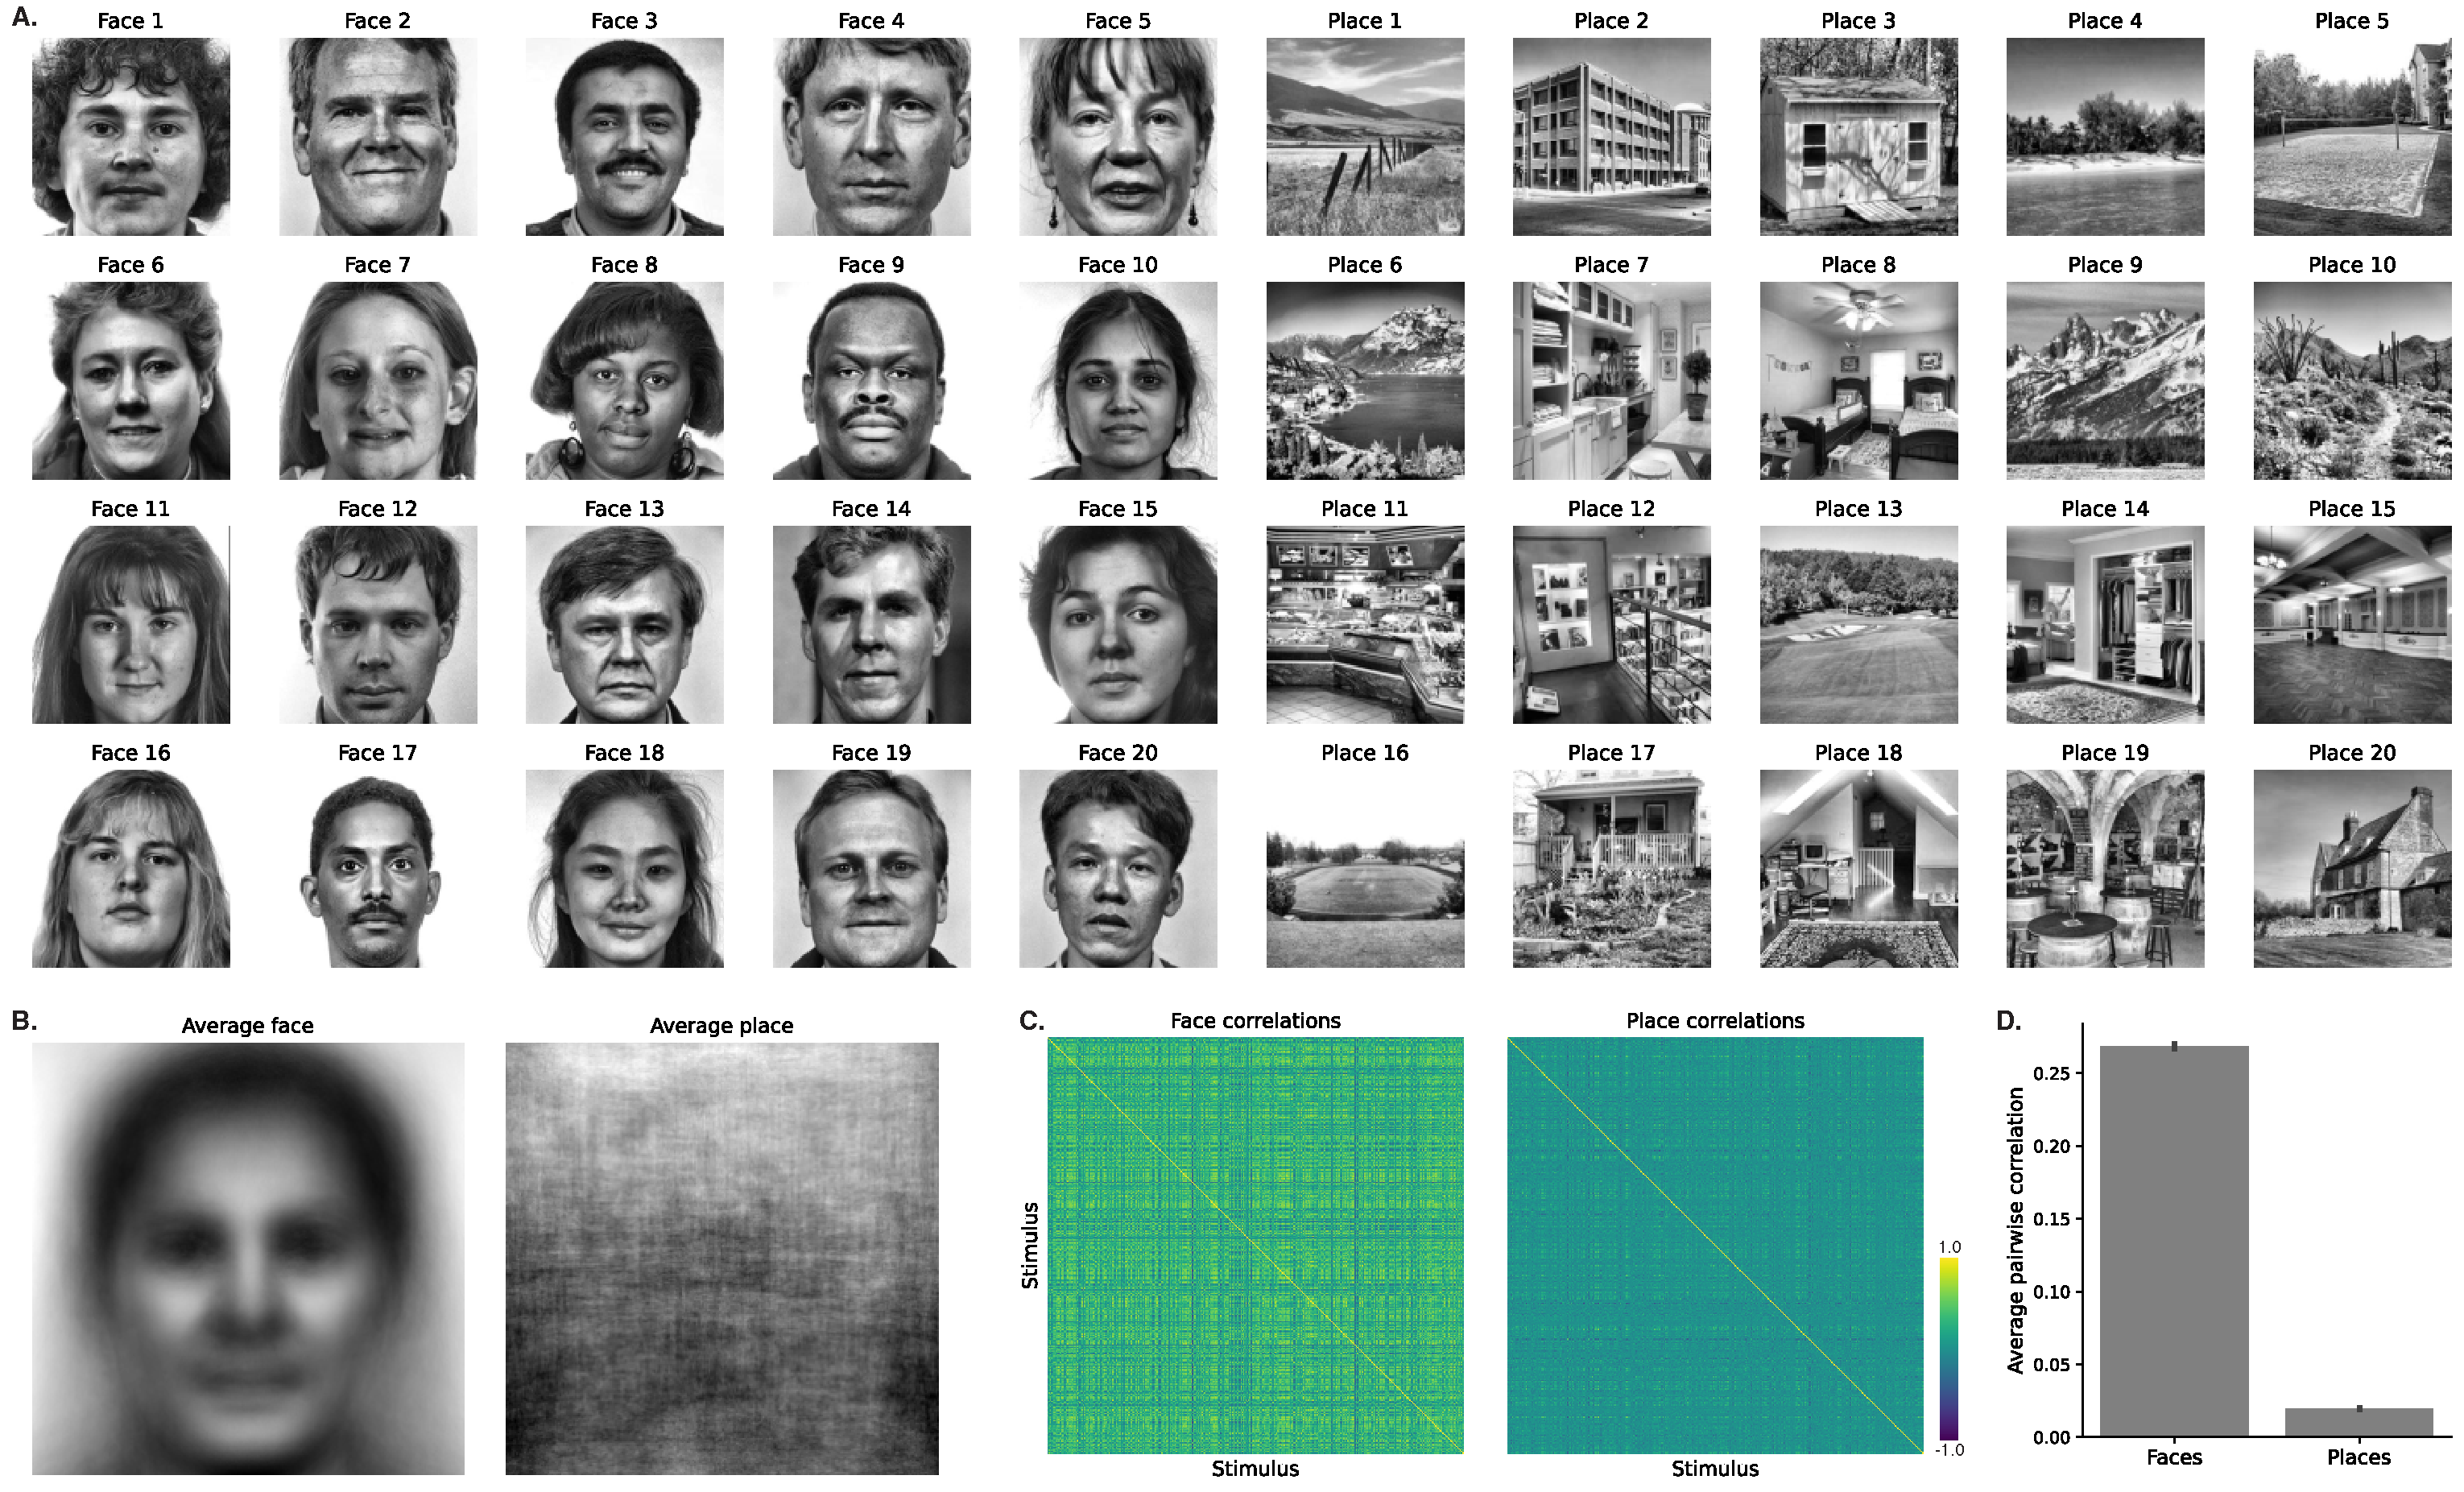
\includegraphics[width=\textwidth]{figs/stimuli}
  
  \caption{\textbf{Stimulus examples and properties.} \textbf{A. Example images
  from each stimulus category.} Randomly chosen subsets of 20 face images
  (left) and 20 place images (right) are displayed. \textbf{B. Across-image
  averages.} Each panel displays the average image, taken across all 360 face
  images (left) and 360 place images (right). \textbf{C. Pairwise
  correlations.} Each row and column of the matrices displays the correlation
  (across pixels) in intensity values for one pair of face images (left) or
  place images (right). \textbf{D. Average pairwise correlations.} The bar
  heights denote the average pairwise correlations between face and place
  images. Error bars denote across-pair bootstrap-estimated 95\%
  confidence intervals.}
  
  \label{fig:stimuli}
  \end{figure*}

Next, we turned to identifying potential differences in participants' behaviors
across the two experimental conditions. The main difference between the
conditions' procedures was in how long participants were asked to maintain the
same focus of category-based and location-based attention, across successive
image presentations. Therefore, differences in participants' behaviors across
the two conditions might reflect differences in the timescales of the relevant
cognitive processes. We compared participants' familiarity ratings for images
at each attention level across the two conditions. We saw no evidence that
people rated fully attended images ($t(51) = -0.649, p = 0.519$),
attended-category (but not location) images ($t(51) = 1.163, p = 0.250$),
unattended category and location images ($t(51) = -1.600, p = 0.116$), or novel
images ($t(51) = -0.435, p = 0.665$) differently across the two conditions.
However, participants in the variable attention condition rated
attended-location (but unattended category) images as more familiar than
participants in the sustained attention condition ($t(51) = 2.174, p = 0.034$).
This suggests that location-based versus category-based attention may operate
over different timescales.

\textbf{JRM STOPPED HERE}

% We considered each image we probed in the memory phase with respect to whether
% (and how) the participant had experienced and/or attended to that image during
% the presentation phase (Fig.~\ref{fig:familiarity}). For example, if a given
% face image had been presented as part of the composite image on the right of
% the screen following an \texttt{attend to the face on the right} instruction,
% then that face image would have been the focus of the participant's attention
% during one stimulus presentation. The face image on the left (unattended side)
% during that trial would have been captured by feature-based attention, but not
% by location-based attention; and the place image (unattended category) on the
% right during that trial would have been captured by location-based attention,
% but not by feature-based attention. The place image on the left during that
% trial remained outside of the focus of both feature-based and location-based
% attention. In this way, we categorized each of the images that participants
% experienced during the presentation phases of each experiment in terms of
% whether they fell under the scope of feature-based and/or location-based
% attention. We also categorized novel face and place images that we asked
% participants to judge during the memory phase (i.e., images that the
% participant hadn't seen before) as belonging to the attention-cued or uncued
% category. These novel images were intended to serve as a baseline for
% comparison. For example, we sought to measure how people rated the familiarity
% of new images in general. We also used differences in familiarity ratings
% between novel images of the attention-cued versus uncued categories to evaluate
% potential \textit{prospective} affects of modulating the focus of feature-based
% attention.

% \begin{figure*}[tp]
%   \centering
%   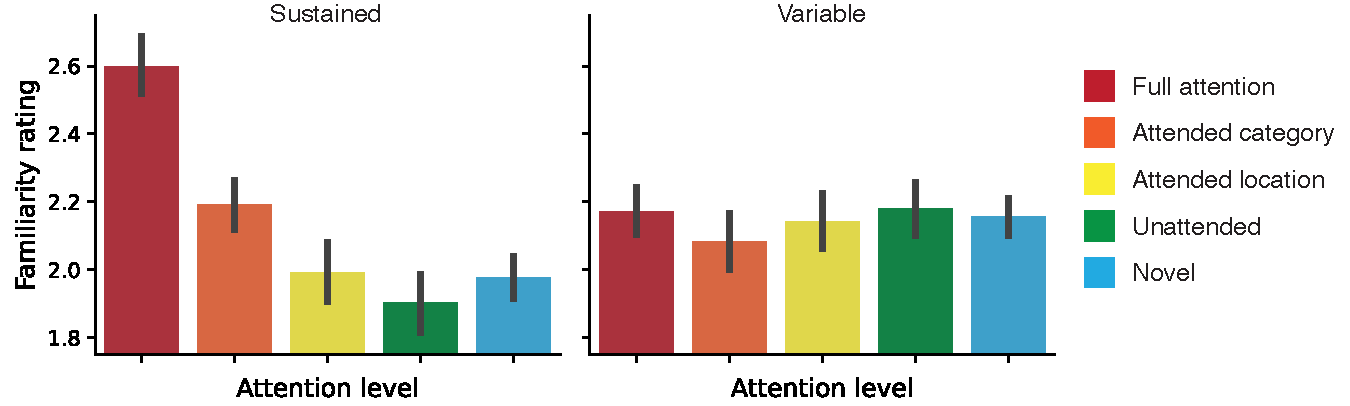
\includegraphics[width=0.75\textwidth]{figs/familiarity_by_attention_level}

%   \caption{\textbf{Familiarity ratings for attended, unattended, and novel
%   stimuli.} The bars display the average familiarity ratings participants gave
%   to images from the same category and location as the attention cue (full
%   attention), the same category (but opposite location) as the attention cue
%   (attended category), the same location (but opposite category) as the
%   attention cue (attended location), the opposite category and location as the
%   attention cue (unattended), or novel images. The left panel displays
%   familiarity ratings from the sustained attention condition and the right
%   panel displays familiarity ratings from the variable attention condition. All
%   error bars denote across-participant bootstrap-estimated 95\% confidence
%   intervals. See Figure~\ratingsByCategory~for analogous results broken down by
%   stimulus category.}

% \label{fig:familiarity}
% \end{figure*}

% Participants in both experiments rated stimuli they attended as more familiar
% than unattended or novel stimuli (Fig.~\ref{fig:familiarity}; Sustained
% Attention Experiment: $t(59) = 13.42, p = 1.39 \times 10^{-19}, d = 1.73$;
% Variable Attention Experiment: $t(52) = 12.40, p = 3.70 \times 10^{-17}, d =
% 1.70$). Participants in both experiments also rated attended scene stimuli as
% more familiar than attended face stimuli (Sustained Attention Experiment:
% $t(59) = 7.69, p = 1.85 \times 10^{-10}, d = 0.99$; Variable Attention
% Experiment: $t(52) = 7.08, p = 3.63 \times 10^{-9}, d = 0.97$). These findings
% indicate that aspects of experience that are captured by the focus of attention
% are easier to recognize later, and that attention may preferentially benefit
% memory for some aspects of experience to a greater extent than other aspects of
% experience.

% Participants in the Sustained Attention Experiment experiment also rated
% unattended images that matched the attended category as more familiar than
% unattended images that did not match the attended category (\textit{incidental
% feature-based attention}; $t(59) = 7.17, p = 1.40 \times 10^{-9}, d = 0.93$).
% This pattern did not hold for participants in the Variable Attention Experiment
% ($t(52) = 0.44, p = 0.66, d = 0.06$). Participants in both experiments
% displayed an incidental effect of location-based attention, whereby they rated
% unattended-category images at the attended location as more familiar than
% unattended-category images at the unattended location (Sustained Attention
% Experiment: $t(59) = 4.32, p = 6.05 \times 10^{-5}, d = 0.56$; Variable
% Attention Experiment: $t(52) = 2.57, p = 0.01, d = 0.35$). This indicates that
% aspects of our experience that incidentally overlap with the focus of our
% location-based attention are easier to recognize later, even if those aspects
% do not fall within the intentional focus of our feature-based attention.

% We defined the \textit{memory benefit of feature-based attention} as the
% difference in mean familiarity ratings of attended stimuli and unattended
% stimuli from the attended category versus the mean familiarity ratings of
% unattended stimuli from the unattended category. Similarly, we defined the
% \textit{memory benefit of location-based attention} as the difference in mean
% familiarity ratings of attended stimuli and unattended stimuli from the
% attended location versus the mean familiarity ratings of unattended stimuli
% from the unattended location. Participants in the Sustained Attention
% Experiment displayed a larger memory benefit of feature-based attention than
% location-based attention ($t(59) = 3.25, p = 1.91 \times 10^{-3}, d = 0.42$),
% whereas participants in the Variable Attention Experiment displayed a larger
% memory benefit of location-based attention ($t(52) = 1.70, p = 9.99 \times
% 10^{-2}, d = 0.23$). This appeared to be driven in part by a response bias
% towards attended-category images. For example, relative to the most recent
% attention cue, participants in the Sustained Attention Experiment rated
% attended-category novel images as more familiar than unattended-category novel
% images ($t(59) = 7.04, p = 2.35 \times 10^{-9}, d = 0.91$), whereas
% participants in the Variable Attention Experiment responded similarly to
% attended-category and unattended-category novel images ($t(52) = 0.23, p =
% 0.82, d = 0.03$). The size of this attended-category response bias for novel
% images was reliably smaller than the memory benefits of feature-based attention
% in both experiments (Sustained Attention Experiment: $t(59) = 7.59, p = 2.68
% \times 10^{-10}, d = 0.98$; Variable Attention Experiment: $t(52) = 6.74, p =
% 1.31 \times 10^{-8}, d = 0.93$). This indicates that tuning the focus of
% feature-based attention with respect to how ongoing experience is encoded in
% memory takes longer than the duration of a single stimulus presentation
% (including fixation, roughly 5.5~s). Further, once feature-based attention
% comes ``online,'' it affects how \textit{new} stimuli are processed.

% We also compared the relative sizes of the memory benefits of feature-based
% attention and location-based attention across the two experiments. Participants
% in the Sustained Attention Experiment displayed a larger difference between
% these two effects than did participants in the Variable Attention Experiment
% ($t(111) = 3.48, p = 7.24 \times 10^{-4}, d = 0.66$). Further, the difference
% in mean familiarity ratings of attended-location images versus unattended
% images was greater for participants in the Variable Attention Experiment
% ($t(111) = 2.32, p = 0.02, d = 0.44$). The memory benefit of location-based
% attention reliably distinguished between attended-category versus unattended
% category images for participants in both experiments (Sustained Attention
% Experiment: $t(59) = 9.50, p = 1.68 \times 10^{-13}, d = 1.23$; Variable
% Attention Experiment: $t(52) = 9.72, p = 2.76 \times 10^{-13}, d = 1.33$). This
% indicates that tuning the focus of location-based attention with respect to how
% ongoing experience is encoded into memory occurs faster than the duration of a
% single stimulus presentation.

% We also compared reaction times to probes from the attended versus unattended
% side. Participants in both experiments responded slightly faster on average to
% attended-side probes, although the differences did not reach significance
% (Sustained Attention Experiment: $t(59) = 1.03, p = 0.31, d = 0.13$; Variable
% Attention Experiment: $t(52) = 0.65, p = 0.52, d = 0.09$). Participants in the
% Sustained Attention Experiment displayed a slightly larger (and not
% statistically significant) difference in attended-side versus unattended-side
% reaction times than participants in the Variable Attention Experiment ($t(111)
% = .87, p = 0.38, d = 0.20$). Because none of these reaction time effects were
% statistically reliable, we are unable to draw meaningful conclusions about
% reaction times to the attention probes on the attended versus unattended side,
% nor are we able to draw meaningful conclusions about differences in those
% reaction times that might be due to sustained versus variable attention.


% \begin{figure}[tp]
%   \centering
%   \includegraphics[width=\textwidth]{figures/exps1_2_xgaze.pdf}

%   \caption{\textbf{Horizontal coordinates of visual fixations.} Each violin
%   plot displays a distribution of participant-wise average horizontal gaze
%   positions relative to a presented image. The coordinates have been normalized
%   such that a value of 1.0 denotes the furthest onscreen coordinate from the
%   central fixation point \textit{towards} the direction of the given image, and
%   -1.0 denotes the furthest onscreen coordinate from the central fixation point
%   \textit{away from} the direction of the given image. The gray bars in each
%   panel mark the boundaries of the presented images. The violin plots are
%   broken down by participants' familiarity ratings during the memory phases of
%   each experiment, and by each image's relation to the attention cue while that
%   image appeared onscreen. Panel \textbf{a.} displays fixation data for the
%   Sustained Attention Experiment and Panel \textbf{b.} displays fixation data
%   for the Variable Attention Experiment. Figure~\fixation~displays these
%   results broken down by participant cohort.}

% \label{fig:fixation}
% \end{figure}


% Given that participants in both experiments rated attended-location images from
% both the attended and unattended category as more familiar than
% unattended-location images, we wondered whether this was truly a consequence of
% covert attention, or whether it might be driven solely by where participants
% were looking. In other words, we sought to distinguish the memory effects of
% the focus of covert attention from the focus of visual gaze. We used
% eyetracking to measure the horizontal positions of the participants' visual
% fixations while each pair of composite stimuli appeared onscreen
% (Fig.~\ref{fig:fixation}). For 94\% of presentation trials (Sustained Attention
% Task: $\frac{4531}{4800}$ trials; Variable Attention Task: $\frac{3972}{4240}$
% trials), we collected viable gaze data for analysis. In the remaining trials,
% participant movement or other technical issues corrupted the gaze data. We
% found that, though they generally followed our instruction to keep their gaze
% fixed on the center of the screen, participants in both experiments exhibited a
% slight tendency to look towards the side of the screen they were attending to
% (Sustained Attention Task: $t(59) = 3.61, p = 6.31 \times 10^{-4}$; Variable
% Attention Task: $t(52) = 2.86, p = 6.06 \times 10^{-3}$). When we limited our
% analyses to trials with viable gaze data where participants successfully
% maintained fixation on the center of the screen within 4.28$^\circ$ visual
% angle (i.e., between the rightmost boundary of the left image and the leftmost
% boundary of the right image) we observed (numerical) memory benefits of
% feature-based attention in both experiments (Sustained Attention Experiment:
% $t(59) = 4.73, p = 1.96 \times 10^{-5}, d = 0.67$; Variable Attention
% Experiment: $t(52) = 0.64, p = 0.52, d = 0.09$) and location-based attention in
% the Sustained Attention Experiment, but not the Variable Attention Experiment
% (Sustained Attention Experiment: $t(59) = 0.67, p = 0.51, d = 0.09$; Variable
% Attention Experiment: $t(52) = -0.79, p = 0.43, d = 0.11$). These analyses
% indicate that although the focus of covert attention can affect where people
% are looking, covert attention affects memory encoding beyond what may be
% accounted for by gaze position alone.


% The preceding results indicate that volitional covert attention affects memory,
% and that feature-based and location-based covert attention may come online at
% different timescales. We next sought to examine how long the memory effects of
% feature-based and location-based covert attention persist. To gain additional
% insights into the timecourse of the impact of feature-based and location-based
% attention on memory, we used a sliding window analysis to measure how
% participants' familiarity ratings of attended, partially attended, unattended,
% and novel stimuli varied over the duration of the memory phases of both
% experiments. During each block within the memory phases of each experiment,
% participants made familiarity judgements about a total of 40 images (20 old
% images and 20 novel images). We computed average familiarity ratings for images
% appearing in each position of the memory stimulus sequence (positions 1--40),
% as a function of how (or whether) they were attended during the preceding
% presentation phase (old images) or whether they matched the category of the
% most recent attention cue (novel images), for overlapping 20-image sliding
% windows (Figs.~\ref{fig:familiarity_timecourse_category},
% \ref{fig:familiarity_timecourse_location}, and
% \ref{fig:familiarity_timecourse_novel}). We first calculated these values for
% each participant, and then we averaged across participants.

% \begin{figure*}[tp]
%   \centering
%   \includegraphics[width=1\textwidth]{figures/Cat_Cued_TimeSeries.pdf}

%   \caption{\textbf{Familiarity ratings over time for images that matched the
%   cued or uncued image category.} Each curve reflects the average familiarity
%   ratings for attended, unattended, and novel images (denoted in the legends on
%   the right) within a succession of overlapping 20-image sliding windows. Error
%   ribbons denote 95\% confidence intervals, computed across participants.
%   Panels \textbf{a.} and \textbf{c.} display results from the Sustained
%   Attention Experiment and Panels \textbf{b.} and \textbf{d.} display results
%   from the Variable Attention Experiment. The paired horizontal lines at the
%   bottom of each panel denote timepoints when the given pair of curves was
%   statistically distinguishable (i.e., the topmost line color was statistically
%   greater than the bottommost line color at $\alpha = 0.05$, via a paired
%   two-tailed $t$-test.) The gray lines in Panels b and d reflect familiarity
%   ratings of novel stimuli from both the most recently attended and unattended
%   image categories. Figures~\timecourseCuedCategory~and
%   \timecourseUncuedCategory~display these results broken down by participant
%   cohort.}

% \label{fig:familiarity_timecourse_category}
% \end{figure*}

% Throughout the memory phase, participants from both experiments rated attended
% images as more familiar than category-matched unattended and novel images
% (Fig.~\ref{fig:familiarity_timecourse_category}, top row). This indicates that
% the memory benefits of attending to specific stimulus features (versus
% category-general features) persist for at least as long as the duration of the
% memory phase (2~min). Early in the memory phase, participants in the Variable
% Attention Experiment also rated category-matched unattended images as more
% familiar than novel images. This pattern did not hold for participants in the
% Sustained Attention Experiment. The short-lived boost in familiarity for
% attended-category images at the unattended location following variable (but not
% sustained) attention suggests that the timecourse of feature-based attention's
% impact on memory depends on how long the focus of feature-based attention has
% been held.

% Participants in both experiments also rated unattended-category images at the
% attended location as more familiar than unattended-category images at the
% unattended location and novel unattended-category images
% (Fig.~\ref{fig:familiarity_timecourse_category}, bottom row). This pattern
% persisted throughout the memory phases of both experiments. This supports the
% notion that location-based attention enhances memory in a (partially)
% feature-independent way. Participants in the Variable Attention Experiment also
% rated unattended-category images at the unattended location as (numerically)
% more familiar than novel images (though this pattern was only statistically
% reliable towards the middle of the memory phase). This pattern did not hold for
% participants in the Sustained Attention Experiment. Participants in the
% Sustained Attention Experiment rated unattended-category images (regardless of
% location or novelty status) as less familiar than participants in the Variable
% Attention Experiment (e.g., compare heights of the lines in the bottom left
% versus bottom right panels of Fig.~\ref{fig:familiarity_timecourse_category}).
% This suggests that, after sustained feature-based attention to a particular
% image category, the encodings of stimuli from the unattended category are
% suppressed. This suppression effect appears to persist at least as long as the
% memory phase of the experiment (2~min). Further, the magnitude of this
% suppression effect appears to become stronger following longer-term sustained
% (versus shorter-term variable) feature-based attention.

% \begin{figure*}[tp]
%   \centering
%   \includegraphics[width=\textwidth]{figures/Side_Cued_TimeSeries_2.pdf}

%   \caption{\textbf{Familiarity ratings over time for images that matched the
%   cued or uncued image location.} This figure follows the same format and
%   conventions as Figure~\ref{fig:familiarity_timecourse_category}.
%   Figures~\timecourseCuedLocation~and \timecourseUncuedLocation~display these
%   results broken down by participant cohort.}

% \label{fig:familiarity_timecourse_location}
% \end{figure*}

% We next examined how participants' familiarity ratings varied over the duration
% of the memory phases of each experiment as a function of the attended location.
% Participants in the Sustained Attention Experiment rated attended-category
% images as more familiar, at both the attended and unattended locations
% (Fig.~\ref{fig:familiarity_timecourse_location}, left panels). In contrast,
% participants in the Variable Attention Experiment rated attended-category
% images as more familiar than unattended-category images only at the attended
% locations (Fig.~\ref{fig:familiarity_timecourse_location}, right panels). The
% primary difference in familiarity ratings between Sustained Attention
% Experiment versus Variable Attention Experiment participants was in how they
% rated unattended-category images. Participants in the Variable Attention Task
% rated unattended-category images as more familiar than did participants in the
% Sustained Attention Task; this pattern persisted throughout the memory phase
% and held for images at both the attended and unattended locations (compare
% heights of blue lines in the left versus right panels of
% Fig.~\ref{fig:familiarity_timecourse_location}). This suggests that lower
% familiarity ratings of unattended-category stimuli in the Sustained Attention
% Experiment are due to suppression of the encoding of unattended-category
% features (e.g., as opposed to enhancement of the encoding of attended-category
% features). This suppression effect appears to build over an interval that is
% longer than the duration of a single stimulus presentation (5.5~s).

% \begin{figure*}[tp]
%   \centering
%   \includegraphics[width=1\textwidth]{figures/Novel_Timecourse_Panels.pdf}

%   \caption{\textbf{Familiarity ratings over time for attended-category and
%   unattended-category novel images.} The top panels of this figure follow the
%   same formats and conventions as
%   Figures~\ref{fig:familiarity_timecourse_category} and
%   \ref{fig:familiarity_timecourse_location}. The bottom panels display the
%   differences between the timecourses of familiarity ratings of
%   attended-category and unattended-category novel stimuli. The error ribbons
%   denote 95\% confidence intervals, computed across participants. The dotted
%   horizontal line in each panel denotes a difference of 0-- i.e., the value
%   above which attended-category novel images were rated as more familiar than
%   unattended-category novel images. The black lines in the bottom panels
%   display linear regression fits to the data (error ribbons denote 95\%
%   confidence intervals). Figures~\timecourseNovel~and \timecourseDiff~display
%   these results broken down by participant cohort.}

% \label{fig:familiarity_timecourse_novel}
% \end{figure*}


% Finally, we examined how participants in both experiments rated the familiarity
% of novel images. These ratings provide insights into how modulating the focus
% of attention to \textit{prior} stimuli can affect the perception of
% \textit{future} stimuli. We considered how participants rated novel stimuli
% that matched versus did not match the category (face or scene) of the most
% recent attention cue. Participants in the Sustained Attention Experiment rated
% attended-category novel stimuli as more familiar than unattended-category novel
% stimuli throughout the entire memory phase
% (Fig.~\ref{fig:familiarity_timecourse_novel}a). By contrast, participants in
% the Variable Attention Experiment rated attended-category and
% unattended-category novel images similarly throughout the memory phase
% (Fig.~\ref{fig:familiarity_timecourse_novel}b). The difference in familiarity
% ratings between the two experiments primarily reflects that participants in the
% Variable Attention Experiment rated unattended-category novel images as more
% familiar than did participants in the Sustained Attention Experiment (e.g.,
% compare blue lines in Fig.~\ref{fig:familiarity_timecourse_novel}a versus
% \ref{fig:familiarity_timecourse_novel}b). This may indicate that the processing
% of unattended-category novel stimuli is suppressed following sustained
% attention (e.g., as opposed to enhancing the processing of attended-category
% novel stimuli). The differences in familiarity between attended-category versus
% unattended-category novel images increased slightly but reliably throughout the
% memory phases of both experiments (Fig.~\ref{fig:familiarity_timecourse_novel},
% bottom panels; slope of regression line fit to differences in Sustained
% Attention Experiment: $\beta = 2.05 \times 10^{-3}, p = 1.07 \times 10^{-14} $;
% slope of regression for Variable Attention Experiment: $\beta = 1.54 \times
% 10^{-3}, p = 5.63 \times 10^{-13} $). This might reflect a process whereby the
% suppression of unattended features continues to build for a short duration even
% after the participant stops volitionally focusing on the attended features.


\section*{Discussion}

We ran two covert attention experiments that asked participants to sustain or
vary the focus of their covert attention, respectively. When participants held
the focus of their feature-based (face versus scene) and location-based (left
versus right) attention for a sustained interval, they judged stimuli they had
seen as familiar when they overlapped with respect to the features and
locations they had attended. The increase in familiarity was larger for
attended-feature images than attended-location images. The increase also
extended to novel stimuli from the attended image category. By contrast, when
participants varied the focus of their feature-based and location-based
attention more rapidly, the boost in familiarity for feature-matched stimuli
was smaller than that for location-matched stimuli, and did not extend to novel
stimuli. Our findings suggest that participants were able to more rapidly
modulate their focus of location-based attention than their focus of
feature-based attention. The tuning of location-based attention appears to be
mediated by enhanced encoding and faster processing at the attended location.
The tuning of feature-based attention appears to be mediated by a suppression
in the encoding and processing of unattended stimulus features. This
suppression effect also affects how new stimuli are processed, and it persists
for a longer duration following an interval when the focus of feature-based
attention was held constant over a longer duration. Taken together, our
findings suggest that feature-based and location-based attention are mediated
by different mechanisms and affect memory at different timescales
(Fig.~\ref{fig:model}).

\begin{figure*}[tp]
  \centering 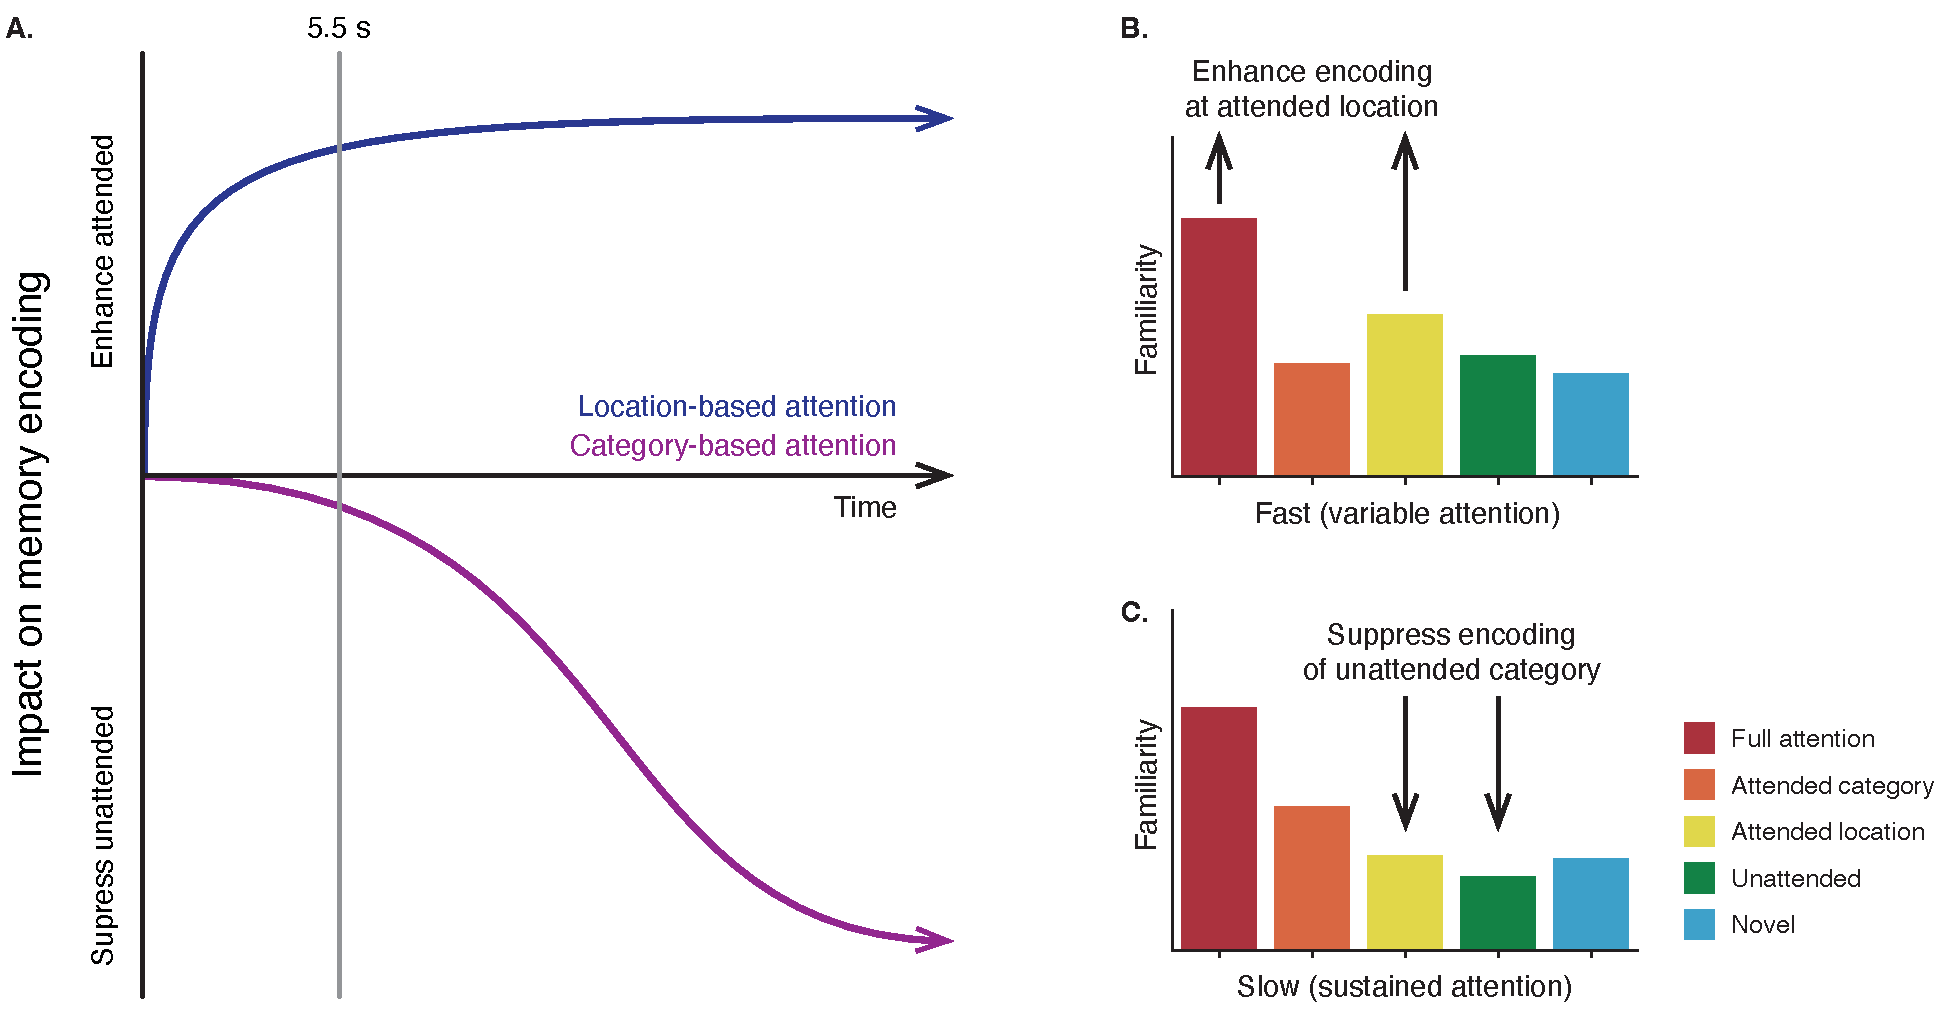
\includegraphics[width=0.75\textwidth]{figures/discussion_schematic}

  \caption{\textbf{Timecourse of encoding and retrieval effects of
  feature-based and location-based attention.} The focus of location-based
  attention (green) may be modulated quickly and rapidly enhances memory
  encoding for nearby stimuli. The focus of feature-based attention (purple) is
  modulated more slowly, and serves to suppress unattended stimulus features.
  The effects of location-based attention on memory persist for longer than the
  effects of feature-based attention. Sustained attention (darker shading)
  yields more robust enhancement and suppression than shorter-term (variable)
  attention (light shading). The vertical gray line on the left denotes the
  duration of a single stimulus presentation (the upper bound by which
  location-based attention begins to affect encoding, and the lower-bound by
  which feature-based attention begins to affect encoding). The vertical gray
  line on the right separates encoding from immediate subsequent retrieval of
  the encoded information.}

\label{fig:model}
\end{figure*}

The notion that location-based attention operates at a faster timescale than
feature-based attention is supported by prior work on the deployment of visual
attention~\citep{SotoBlan04, StopEtal07}. Our findings that location-based
attention enhances the processing of attended stimuli whereas feature-based
attention suppresses the processing of unattended stimuli is also consistent
with prior work on location-based attention~\citep[e.g.,][]{IttiKoch01} and
feature-based attention~\citep[e.g.,][]{MoheEtal14}. Our finding that people
better remember attended stimuli also follows prior work on interactions
between attention and memory~\citep{PallWagn02, ChunTurk07, AlyTurk16,
AlyTurk17, WittEtal18, MorrEtal14, BaleEtal19}. Whereas much of this prior work
focused on elucidating the neural basis of these interactions, our work extends
these prior studies by elucidating the specific and separable behavioral
impacts of feature-based attention (inhibition with a slow onset) and
location-based attention (enhancement with a fast onset) on subsequent memory.
Both of these effects persisted throughout the 2~min memory phases of both
experiments. Therefore future work is needed to elucidate the longevity of
these effects beyond 2 minutes.

Another important area for future study concerns how the flow of information
between different brain structures is modulated according to the focus of
volitional attention-- particularly with respect to pathways from primary
sensory regions (e.g., V1, A1) to regions implicated in encoding ongoing
experiences into memory (e.g, medial temporal lobe structures such as the
hippocampus and entorhinal cortex, prefrontal cortex, etc.). For example,
several studies suggest that attention serves to modulate the \textit{gain} of
specific neural circuits~\citep{TreuTruj99, ChanEtal02, EldaEtal13,
SaliThie00}, effectively facilitating or inhibiting the flow of specific neural
representations~\citep{VartEtal07, LaRoEtal14}. Prior work suggests that
feature-based attention may be supported by changes in connectivity with the
thalamus~\citep{Schn11}, whereas location-based attention may be supported by
changes in connectivity with primary visual cortex~\citep{NoudEtal10}. That
feature-based and location-based attention are mediated by different brain
structures may explain why these different aspects of attention operate on
different timescales and affect memory differently. A strong test of this
hypothesis would entail directly measuring neural activity patterns as people
modulate their focus of attention (e.g., using functional magnetic resonance
imaging or electroencephalography), and then using neural decoding
approaches~\citep[e.g.,][]{HaxbEtal01, NormEtal06, MannEtal18} to follow how
neural representations of attended (or unattended) stimuli are transfered from
primary sensory regions, to higher order sensory regions, to memory areas. If
the effects of attention on memory are mediated by changes in network dynamics,
the transmission rates of the representations of attended stimuli from primary
sensory regions to memory areas should be facilitated relative to the
transmission rates of unattended stimuli. Further, variability in these neural
changes (e.g., as a participant focuses their attention with more or less
success) should track with behavioral measures of memorability.

Which aspects of our ongoing experiences we choose to attend affects how we
process and remember those experiences later. Different forms of
attention---e.g., to specific features or spatial locations---operate and
affect memory at different timescales, and are likely mediated by different
brain networks. Elucidating the behavioral and neural consequences of
volitional changes in attention is central to discovering how our thoughts,
feelings, goals, and situational understanding fluctuate from moment to moment.


\section*{Author Contributions}

JRM and KZ developed the concept for this study. Experiment code was written by
KZ and ARM, and testing and data collection were conducted by MRL and KZ. KZ,
MRL, ARM, and JRM analyzed the data. JRM supervised the project. All authors
contributed to writing and editing the manuscript.

\section*{Data and code availability}

All of the data analyzed in this manuscript, along with all of the code for
running our experiment and carying out the analyses may be found at
\url{http://www.github.com/ContextLab/attention-memory-task}.


\section*{Acknowledgements}

This work was supported in part by NSF EPSCoR Award Number 1632738 to JRM and
by by NSF CAREER Award Number 2145172 to JRM. The content of this manuscript is
solely the responsibility of the authors and does not necessarily represent the
official views of our supporting organizations. We are grateful for useful
discussions with the EPSCoR Attention Consortium, particularly with Marian
Berryhill, Gideon Caplovitz, Patrick Cavanagh, Theresa Desrochers, and Peter
Tse. We thank Megan deBettencourt for useful discussions, pointers to our
experimental stimuli, and for providing code to facilitate stimulus
preparation. We also appreciate useful discussions with Paxton Fitzpatrick,
Kevin Hartstein, Talia Manning, Lucy Owen, and Michael Ziman. Finally, we thank
Christina Liu and Eowyn Pak for their help running pilot versions of the
experiments reported here.


\bibliographystyle{apacite}
\bibliography{./CDL-bibliography/memlab}



\end{document}
